
\chapter{Instruccions generals i itinerari del Treball Final de Grau }\label{instruccions}
\begin{figure}
\centering
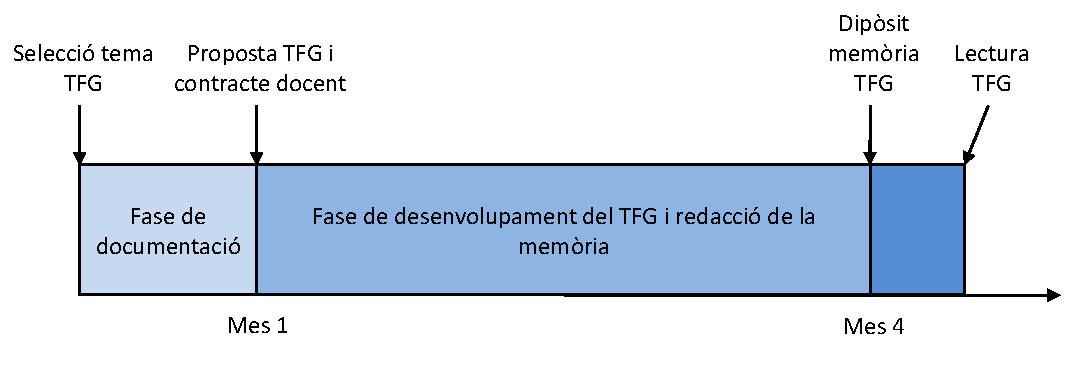
\includegraphics[width=\linewidth]{Itinerari_TFG}
\caption{\label{fig:itinerari}Itinerari del TFG}
\end{figure}
\section{Introducci }
A continuaci  es descriuen les passes que heu de seguir per a la realitzaci  del vostre TFG. Una vegada llegit aquest cap tol ens conv  consultar la normativa de TFG  de l'EPS on trobarem una informaci  m s detallada.
\section{Inici del TFG}

Com a norma general, tal com apareix reflectit en els plans d'estudis de gaireb  totes les titulacions de grau, el TFG s'hauria de realitzar en el segon semestre de quart curs.  Aix  doncs, atesa la naturalesa integradora del TFG, la normativa de l'EPS especifica que ens podrem matricular del TFG sempre que estiguem matriculats de tots els cr dits necessaris per a l'obtenci  del t tol corresponent.  
\section{Selecci  del tema de TFG}

Una de les vies m s habituals per escollir el tema de TFG  s a trav s de l'apartat corresponent de la web de l'Escola Polit cnica Superior (EPS). En aquest cas, despr s de revisar les propostes realitzades pels diferents professors o grups de recerca involucrats en la doc ncia de l'EPS, escollirem les que m s ens interessin i contactarem amb els professors responsables fins que algun dels professors que encara no tingui el tema assignat ens accepti. %Si algun dels professors encara no t  el tema assignat i ens accepta, comen arem a treballar en la fase de documentaci  i en la preparaci  de la proposta.

Existeixen altres possibilitats a l'hora d'escollir un tema de TFG. Per exemple, es pot donar el cas d'alumnes que prefereixin realitzar el TFG en una empresa o alumnes que estiguin especialment interessats en un  rea de coneixement concreta i ells mateixos vulguin proposar un tema de TFG. En qualsevol d'aquests casos  s important que trobeu un tutor a l'universitat que trameti la proposta de tema de TFG i que es comprometi a dirigir el vostre treball. En el cas de TFGs desenvolupats en empreses ser  important tamb  comptar amb el vist-i-plau del supervisor dintre de l'empresa. En cas de dubte, el m s convenient  s contactar amb el cap d'estudis de la titulaci  corresponent que segur que ens orientar  i ens proporcionar  la informaci  necess ria.

Val a dir que el TFG tamb  es pot realitzar en una universitat amb la que s'hagin establert convenis de convalidaci  (programes S neca, Erasmus, Averroes, \ldots). Tanmateix, en aquest cas haurem de seguir els procediments administratius establerts en aquesta altra universitat.

\section{Inscripci  de la sol licitud de TFG i contracte docent}

Un cop escollit el tema hem d'inscriure el nostre TFG lliurant l'impr s de sol licitud juntament amb el nostre tutor a trav s de l'espai dedicat als TFG de Campus Extens.  La sol licitud inclou un contracte docent en el que s'establiran els compromisos del professor quant a seguiment i supervisi  del TFG i els de l'estudiant quant a dedicaci  i termini de presentaci .  Una vegada que la nostra sol licitud hagi estat aprovada pel cap d'estudis de la nostra titulaci  aquest tema de TFG passar  a l'estat d'assignat dins el llistat de temes de TFG. El proc s de selecci  de temes i el lliurament de la sol licitud a la secretaria ha d'acabar en un termini de 20 dies a partir de la data de finalitzaci  del per ode de matr cula.

\section{Desenvolupament del TFG}

El desenvolupament del TFG comen a habitualment per una fase de documentaci  a on el nostre tutor ens proporcionar  la informaci  necessaria per introduir-nos dins la tem tica del nostre treball. Acabada la fase de documentaci  ens dedicarem a la realitzaci  del TFG i a la redacci  de la mem ria sota la supervisi  del tutor i seguint les condicions estipulades en el contracte docent. Per a la redacci  de la mem ria conv  seguir les indicacions descrites al cap tol \ref{mem ria} i el format proporcionat a la plantilla i l'ap ndix d'aquest document, exceptuant en el cas de projectes t cnics (projectes de rehabilitaci  d'edificis, projectes d'ajardinament...) on es seguiran les especificacions de la norma UNE 157001:2002 i les recomanacions de les assignatures de projectes dels plans d'estudis corresponents.  s recomanable que aquesta fase de desenvolupament i redacci  del treball, tal com ens mostra la Fig. \ref{fig:itinerari}, no superi els quatre mesos.

\section{Dip sit de la mem ria}

Una vegada acabada la seva redacci  si ja hem superat tots els altres cr dits del pla d'estudis, i amb el vist-i-plau del nostre tutor, dipositarem la mem ria del TFG a secretaria un exemplar en paper i un electr nic seguint les indicacions de format de l'ap ndix A.

\section{Preparaci  de la presentaci }

Finalment nom s ens quedar  preparar la presentaci  del TFG per tal de fer-ne la defensa oral davant el tribunal. Per a la preparaci  d'aquesta presentaci  conv  seguir les indicacions del cap tol \ref{presentaci }.
